\subsection{Section 6.2}

\begin{tcolorbox}[
        title={Problem 10},
        valign=center,
        nobeforeafter,
        colframe=gray!95!black
    ]
    
    Calculate:
    \begin{align}
        \iint_R \frac{1}{x + y} \ dydx
    \end{align}
    
    where \(R\) is the region bounded by \(x = 0\), \(y = 0\), \(x + y = 1\), \(x + y = 4\), by using the mapping \(T(u, v) = (u - uv, uv)\).
\end{tcolorbox}

\begin{solution}
     We first find the bounds of our integral in terms of \(u\) and \(v\). 
    
    We require that:
    \begin{align*}
        x + y &\geq 1 & x + y &\leq 4 \\
        u - uv + uv &\geq 1 & u - uv + uv &\leq 4 \\
        u &\geq 1 & u &\leq 4
    \end{align*}
    This implies that \(1 \leq u \leq 4\).
    
    We also require that:
    \begin{align*}
        x &\geq 0 & y &\geq 0 \\
        u - uv &\geq 0 & uv &\geq 0 \\
        u &\geq uv & v &\geq 0 \\
        1 &\geq v
    \end{align*}
    This implies that \(0 \leq v \leq 1\).
    
    We now compute the absolute value of the Jacobian:
    \begin{align*}
        \left|\frac{\partial(x, y)}{\partial(u, v)}\right| &= \left|\begin{vmatrix}
            \frac{\partial x}{\partial u} & \frac{\partial x}{\partial v} \\
            \frac{\partial y}{\partial u} & \frac{\partial y}{\partial v}
        \end{vmatrix}\right| \\
        &= \left|\begin{vmatrix}
            1 - v & -u \\
            v & u
        \end{vmatrix}\right| \\
        &= \left|(1-v)u + uv\right| \\
        &= \left|u - uv + uv\right| \\
        &= |u| \\
        &= u
    \end{align*}
    where \(|u| = u\) since \(1 \leq u \leq 4\). 
    
   Then the integral in the new coordinate system is given by:
    \begin{align*}
        \iint_R \frac{1}{x + y} \ dydx &= \iint_{R'} \frac{1}{u - uv + uv} \left|\frac{\partial(x, y)}{\partial(u, v)}\right| \ du dv \\
        &= \int_{0}^{1} \int_{1}^4 \frac{u}{u} \ du dv \\
        &= \int_{0}^{1} (4 - 1) \ dv \\
        &= 3 \int_{0}^{1} dv \\
        &= 3
    \end{align*}
\end{solution}

\begin{tcolorbox}[
        title={Problem 36 (a)},
        valign=center,
        nobeforeafter,
        colframe=gray!95!black
    ]
    Let \(R\) denote the region inside \(x^2 + y^2 = 1\), but outside \(x^2 + y^2 = 2y\) with \(x \geq 0\) and \(y \geq 0\). \\
    
    Sketch this region.
\end{tcolorbox}

\begin{solution}
    The region inside \(x^2 + y^2 = 1\) with \(x \geq 0\) and \(y \geq 0\) is given by:
    \begin{figure}[h!]
        \centering
        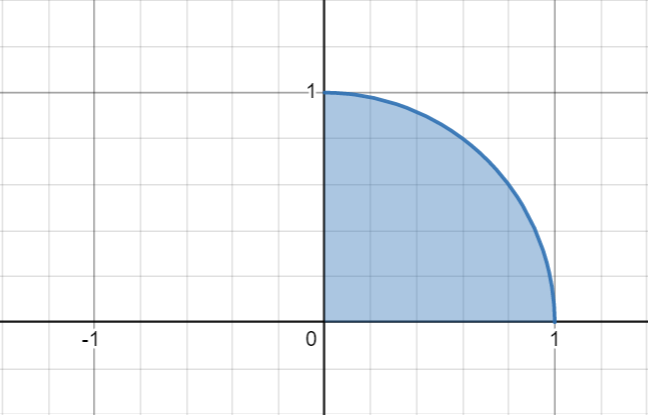
\includegraphics[width=0.6\textwidth]{Pictures/Tutorial 6-1.png}
        \caption{Unit disk centered at the origin, restricted to the first quadrant of the coordinate plane.}
    \end{figure}
    
    The region outside \(x^2 + y^2 = 2y\) requires some manipulation. 
    
    Observe:
    \begin{align*}
        x^2 + y^2 &= 2y \\
        x^2 + y^2 - 2y &= 0 \\
        x^2 + y^2 - 2y + 1 &= 1 \\
        x^2 + (y - 1)^2 &= 1
    \end{align*}
    
    By completing the square, we can see that this constraint takes the form of a unit disk centered at \((x, y) = (0, 1)\). 
    
    The region outside \(x^2 + y^2 = 2y\) with \(x \geq 0\) and \(y \geq 0\) is given by:
    \begin{figure}[h!]
        \centering
        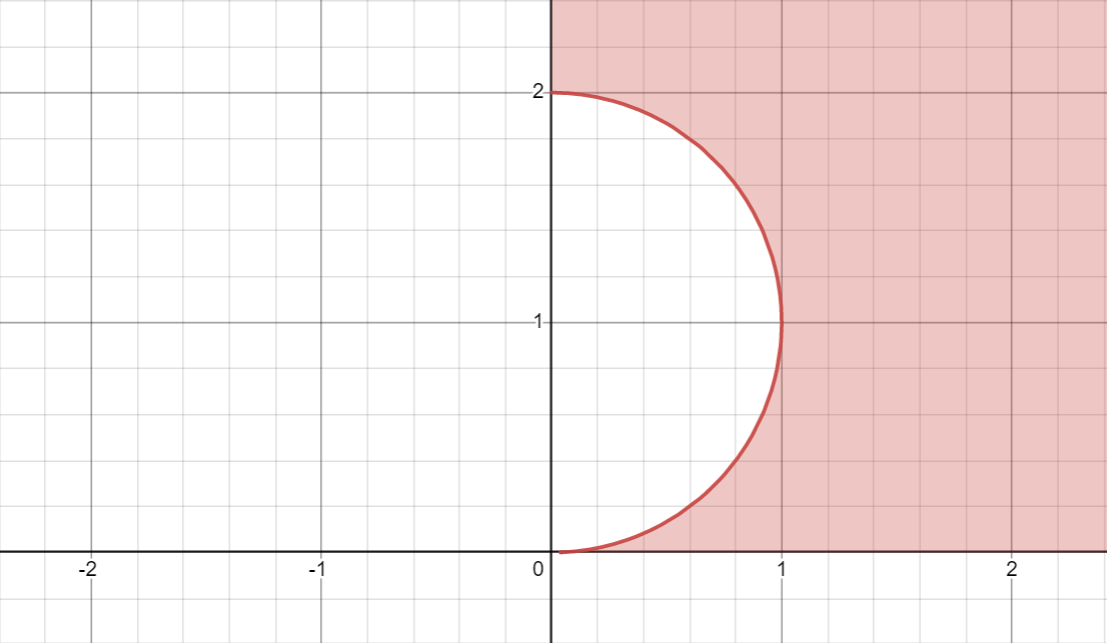
\includegraphics[width=0.6\textwidth]{Pictures/Tutorial 6-2.png}
        \caption{Unit disk centered at the point \((x, y) = (0, 1)\), restricted to the first quadrant of the coordinate plane.}
    \end{figure}
    
    \newpage
    Combined, we obtain the following region:
    \begin{figure}[h!]
        \centering
        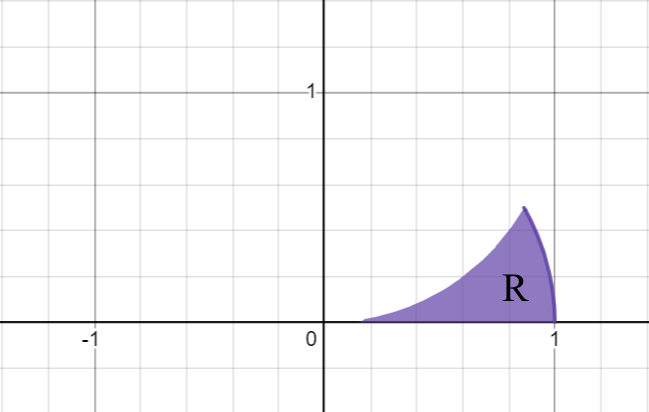
\includegraphics[width=0.6\textwidth]{Pictures/Tutorial 6-3.png}
        \caption{Intersection of the two previous regions.}
    \end{figure}
\end{solution}

\begin{tcolorbox}[
        title={Problem 36 (b)},
        valign=center,
        nobeforeafter,
        colframe=gray!95!black
    ]
    Let \(u = x^2 + y^2\) and \(v = x^2 + y^2 - 2y\). \\
    
    Sketch the region \(R'\) in the \(uv\) plane which corresponds to \(R\) under this change of coordinates.
\end{tcolorbox}

\begin{solution}
    We first isolate for \(y\):
    \begin{align*}
        v &= x^2 + y^2 - 2y \\
        v &= u - 2y \\
        y &= \frac{u - v}{2}
    \end{align*}
    
    We require that:
    \begin{align*}
        x^2 + y^2 &\leq 1 & x^2 + y^2 &\geq 2y\\
        u &\leq 1 & u &\geq u - v \\
        & & 0 &\geq - v \\
        & & v &\geq 0
    \end{align*}
    since \(x^2 + y^2 \geq 0\) always, it follows that \(0 \leq u \leq 1\).
    
    To find the upper bound for \(v\), we also require that \(y \geq 0\):
    \begin{align*}
        y &\geq 0 \\
        \frac{u - v}{2} &\geq 0 \\
        u &\geq v
    \end{align*}
    
    The bounds of our integral in terms of \(u\) and \(v\) should therefore be:
    \begin{align}
        0 \leq &u \leq 1 & 0 \leq v \leq u 
    \end{align}
    
    \begin{figure}[h!]
        \centering
        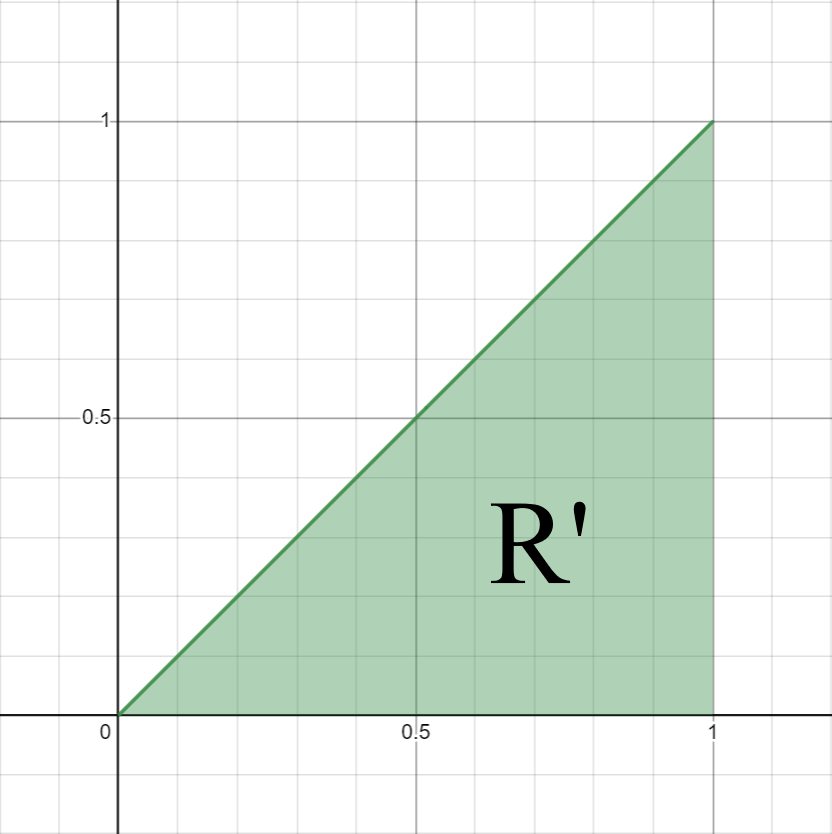
\includegraphics[width=0.4\textwidth]{Pictures/Tutorial 6-4.png}
        \caption{Domain of integration \(R'\) in the \(uv\) plane.}
    \end{figure}
\end{solution}

\begin{tcolorbox}[
        title={Problem 36 (c)},
        valign=center,
        nobeforeafter,
        colframe=gray!95!black
    ]
    Compute:
    \begin{align}
        \iint_R xe^y \ dxdy
    \end{align}
    using the previously mentioned change of coordinates.
\end{tcolorbox}

\begin{solution}
    We first compute the Jacobian:
    \begin{align*}
        \left|\frac{\partial(x, y)}{\partial(u, v)}\right| &= \left|\frac{\partial(u, v)}{\partial(x, y)}\right|^{-1} \\
        &= \left|\begin{vmatrix}
            \frac{\partial u}{\partial x} & \frac{\partial u}{\partial y} \\
            \frac{\partial v}{\partial x} & \frac{\partial v}{\partial y}
        \end{vmatrix}\right|^{-1} \\
        &= \left|\begin{vmatrix}
            2x & 2y \\
            2x & 2y - 2
        \end{vmatrix}\right|^{-1} \\
        &= \left|2x(2y - 2) - 2x(2y)\right|^{-1} \\
        &= \left|4xy - 4x - 4xy\right|^{-1} \\
        &= \left|-4x\right|^{-1} \\
        &= \frac{1}{4|x|} \\
        &= \frac{1}{4x}
    \end{align*}
    where \(|x| = x\) since \(x \geq 0\).
    
    Then the integral in the new coordinate system is given by:
    \begin{align*}
        \iint_R xe^y \ dxdy &= \iint_{R'} xe^{\frac{u - v}{2}} \left|\frac{\partial(x, y)}{\partial(u, v)}\right| \ du dv \\
        &= \frac{1}{4} \int_{0}^{1} \int_{0}^{u} \frac{x}{x}e^{\frac{u - v}{2}} \ du dv \\
        &= \frac{1}{4} \int_{0}^{1} \int_{0}^{u} e^{\frac{u - v}{2}} \ dv du \\
        &= \frac{1}{4} \int_{0}^{1} -2 e^{\frac{u - v}{2}} \Big|_{0}^{u} \ du \\
        &= \frac{1}{4} \int_{0}^{1} -2 e^{0} + 2 e^{\frac{u}{2}} \ du \\
        &= \frac{1}{2} \int_{0}^{1} e^{\frac{u}{2}} - 1 \ du \\
        &= \frac{1}{2} \left( 2 e^{\frac{u}{2}} - u\right)\Big|_{0}^{1} \\
        &= \frac{1}{2} \left( 2 e^{\frac{1}{2}} - 2e^0 - 1\right) \\
        &= \frac{1}{2} \left( 2 e^{\frac{1}{2}} - 3\right) \\
        &= e^{\frac{1}{2}} - \frac{3}{2}
    \end{align*}
\end{solution}